\documentclass[10pt,twocolumn]{article}
\usepackage[margin=0.75in]{geometry}
\usepackage{booktabs,graphicx,amsmath,hyperref,xcolor}
\newcommand{\pending}[1]{\textcolor{red}{[pending: #1]}}
\newcommand{\blipMean}{73.1}
\newcommand{\blipMeanStd}{1.6}
\newcommand{\blipGreedy}{70.2}
\newcommand{\blipGreedyStd}{1.1}
\newcommand{\blipFactF}{80.4}
\newcommand{\blipFactFStd}{0.9}
\newcommand{\blipPresence}{91.7}
\newcommand{\blipIdentify}{69.3}
\newcommand{\blipExtent}{65.1}
\newcommand{\blipLocation}{66.4}
\newcommand{\zeroMean}{29.6}
\newcommand{\zeroMeanStd}{0.4}
\newcommand{\zeroGreedy}{16.4}
\newcommand{\zeroGreedyStd}{0.4}
\newcommand{\zeroFactF}{0.0}
\newcommand{\zeroFactFStd}{0.0}
\newcommand{\zeroPresence}{59.4}
\newcommand{\zeroIdentify}{13.4}
\newcommand{\zeroExtent}{41.1}
\newcommand{\zeroLocation}{4.3}
\newcommand{\voneMean}{67.7}
\newcommand{\voneMeanStd}{0.9}
\newcommand{\voneGreedy}{66.8}
\newcommand{\voneGreedyStd}{0.9}
\newcommand{\voneFactF}{58.3}
\newcommand{\voneFactFStd}{4.0}
\newcommand{\vonePresence}{89.9}
\newcommand{\voneIdentify}{59.3}
\newcommand{\voneExtent}{60.6}
\newcommand{\voneLocation}{60.9}
\newcommand{\vtwoMean}{68.1}
\newcommand{\vtwoMeanStd}{1.2}
\newcommand{\vtwoGreedy}{66.8}
\newcommand{\vtwoGreedyStd}{1.1}
\newcommand{\vtwoFactF}{76.8}
\newcommand{\vtwoFactFStd}{2.7}
\newcommand{\vtwoPresence}{90.5}
\newcommand{\vtwoIdentify}{60.4}
\newcommand{\vtwoExtent}{60.3}
\newcommand{\vtwoLocation}{61.0}
\newcommand{\blipRanked}{73.1}
\newcommand{\finalCycle}{5}
\newcommand{\finalPairs}{960k}
\newcommand{\finalVal}{71.5}
\newcommand{\blipPartial}{77.5}
\newcommand{\finalChange}{1.6}
\newcommand{\finalChangeLo}{0.8}
\newcommand{\finalChangeHi}{2.3}
\newcommand{\finalChangeFolds}{5}
\newcommand{\prevVal}{69.5}
\newcommand{\totalChange}{5.0}
\newcommand{\totalChangeLo}{3.7}
\newcommand{\totalChangeHi}{6.4}
\newcommand{\capChange}{3.6}
\newcommand{\capChangeLo}{1.2}
\newcommand{\capChangeHi}{6.0}
\newcommand{\capChangeFolds}{5}
\newcommand{\blipCorrMean}{74.6}
\newcommand{\blipCorrMeanStd}{1.4}
\newcommand{\corrChange}{1.5}
\newcommand{\corrChangeLo}{0.9}
\newcommand{\corrChangeHi}{2.0}
\newcommand{\corrChangeFolds}{5}
\newcommand{\corrIdentify}{75.1}
\newcommand{\corrNdTrue}{1,353}
\newcommand{\corrNdSaid}{481}
\newcommand{\corrValChange}{1.8}
\newcommand{\corrValLo}{1.2}
\newcommand{\corrValHi}{2.4}
\newcommand{\corrValFolds}{5}
\newcommand{\tfourHours}{64}
\newcommand{\proHours}{114}
\newcommand{\constMean}{42.4}
\newcommand{\constLocation}{57.3}
\newcommand{\constIdentify}{23.2}
\newcommand{\blipAccEighty}{83.9}
\newcommand{\blipAurc}{0.08}
\newcommand{\blipCreditAmb}{39.9}
\newcommand{\blipAccClear}{77.3}
\newcommand{\blipEce}{0.13}
\newcommand{\blipAccAll}{73.5}
\newcommand{\zeroAurc}{0.53}
\newcommand{\leakGap}{$-2.3$}
\newcommand{\leakLo}{$-6.5$}
\newcommand{\leakHi}{2.2}
\newcommand{\leakSeen}{72.3}
\newcommand{\leakUnseen}{74.6}
\newcommand{\ndviDiff}{0.1}
\newcommand{\ndviLo}{$-0.8$}
\newcommand{\ndviHi}{0.9}
\newcommand{\qwenRgbMean}{67.3}
\newcommand{\qwenRgbPooled}{70.3}
\newcommand{\qwenRgbPresence}{81.4}
\newcommand{\qwenRgbLocation}{62.1}
\newcommand{\qwenRgbFactF}{64.9}
\newcommand{\qwenRgbPrecision}{65.9}
\newcommand{\qwenRgbRecall}{64.0}
\newcommand{\qwenRgbDiff}{$-5.1$}
\newcommand{\qwenRgbWords}{9}
\newcommand{\referenceWords}{6}
\newcommand{\qwenNdviMean}{66.9}
\newcommand{\qwenNdviPooled}{70.4}
\newcommand{\qwenNdviPresence}{83.1}
\newcommand{\qwenNdviLocation}{61.5}
\newcommand{\qwenNdviFactF}{65.5}
\newcommand{\qwenNdviPrecision}{63.3}
\newcommand{\qwenNdviRecall}{67.7}
\newcommand{\qwenNdviDiff}{$-5.0$}
\newcommand{\qwenNdviWords}{9}
\newcommand{\blipFoldMean}{71.0}
\newcommand{\blipFoldPooled}{75.4}
\newcommand{\blipFoldPresence}{91.7}
\newcommand{\blipFoldLocation}{66.6}
\newcommand{\blipFoldFactF}{80.3}
\newcommand{\blipFoldPrecision}{78.2}
\newcommand{\blipFoldRecall}{82.5}
\newcommand{\blipFoldWords}{9}
\newcommand{\voneFoldMean}{67.7}
\newcommand{\voneFoldPooled}{72.6}
\newcommand{\voneFoldPresence}{90.5}
\newcommand{\voneFoldLocation}{61.9}
\newcommand{\voneFoldFactF}{61.3}
\newcommand{\voneFoldPrecision}{45.9}
\newcommand{\voneFoldRecall}{92.0}
\newcommand{\voneFoldDiff}{$-2.8$}
\newcommand{\voneFoldWords}{33}
\newcommand{\vtwoFoldMean}{67.6}
\newcommand{\vtwoFoldPooled}{72.5}
\newcommand{\vtwoFoldPresence}{90.6}
\newcommand{\vtwoFoldLocation}{63.3}
\newcommand{\vtwoFoldFactF}{77.3}
\newcommand{\vtwoFoldPrecision}{75.7}
\newcommand{\vtwoFoldRecall}{79.0}
\newcommand{\vtwoFoldDiff}{$-2.9$}
\newcommand{\vtwoFoldWords}{9}
\newcommand{\balancedMean}{66.5}
\newcommand{\balancedPooled}{71.7}
\newcommand{\balancedPresence}{91.0}
\newcommand{\balancedLocation}{56.0}
\newcommand{\balancedFactF}{77.3}
\newcommand{\balancedPrecision}{75.7}
\newcommand{\balancedRecall}{79.0}
\newcommand{\balancedDiff}{$-0.8$}
\newcommand{\balancedWords}{9}
\newcommand{\doraMean}{67.2}
\newcommand{\doraPooled}{72.2}
\newcommand{\doraPresence}{90.5}
\newcommand{\doraLocation}{62.9}
\newcommand{\doraFactF}{61.2}
\newcommand{\doraPrecision}{45.9}
\newcommand{\doraRecall}{92.0}
\newcommand{\doraDiff}{$-0.4$}
\newcommand{\doraWords}{33}
\newcommand{\blipParaphraseDrop}{8.3}
\newcommand{\blipJpegDrop}{24.8}
\newcommand{\blipBlurDrop}{15.6}
\newcommand{\blipNoiseDrop}{10.5}
\newcommand{\blipResDrop}{14.1}
\newcommand{\blipLightDrop}{2.8}
\newcommand{\blipFlipDrop}{0.3}
\newcommand{\blipRotDrop}{2.8}
\newcommand{\blipJpegAcc}{50.5}
\newcommand{\blipRobustClean}{75.3}
\newcommand{\blipPerturbed}{6.9}
\newcommand{\vtwoParaphraseDrop}{10.7}
\newcommand{\vtwoJpegDrop}{14.5}
\newcommand{\vtwoBlurDrop}{11.4}
\newcommand{\vtwoNoiseDrop}{4.7}
\newcommand{\vtwoResDrop}{9.9}
\newcommand{\vtwoLightDrop}{0.4}
\newcommand{\vtwoFlipDrop}{0.1}
\newcommand{\vtwoRotDrop}{0.6}
\newcommand{\vtwoJpegAcc}{57.3}
\newcommand{\vtwoRobustClean}{71.9}
\newcommand{\vtwoPerturbed}{3.9}
\newcommand{\voneParaphraseDrop}{11.3}
\newcommand{\voneJpegDrop}{14.4}
\newcommand{\voneBlurDrop}{9.5}
\newcommand{\voneNoiseDrop}{5.2}
\newcommand{\voneResDrop}{8.1}
\newcommand{\voneLightDrop}{0.6}
\newcommand{\voneFlipDrop}{$-0.0$}
\newcommand{\voneRotDrop}{1.0}
\newcommand{\voneJpegAcc}{57.3}
\newcommand{\voneRobustClean}{71.6}
\newcommand{\vonePerturbed}{3.9}
\newcommand{\servedRgbParaphraseDrop}{7.0}
\newcommand{\servedRgbFlipDrop}{1.2}
\newcommand{\servedRgbRotDrop}{1.9}
\newcommand{\servedNdviParaphraseDrop}{4.2}
\newcommand{\servedNdviFlipDrop}{$-1.0$}
\newcommand{\servedNdviRotDrop}{$-0.8$}
\newcommand{\blipMidJpeg}{12.3}
\newcommand{\blipMidBlur}{9.6}
\newcommand{\blipMidNoise}{4.9}
\newcommand{\blipMidRes}{7.0}
\newcommand{\blipMidLight}{0.6}
\newcommand{\servedRgbMidJpeg}{4.0}
\newcommand{\servedRgbMidBlur}{4.4}
\newcommand{\servedRgbMidNoise}{2.8}
\newcommand{\servedRgbMidRes}{2.1}
\newcommand{\servedRgbMidLight}{2.3}
\newcommand{\servedNdviMidJpeg}{2.3}
\newcommand{\servedNdviMidBlur}{3.4}
\newcommand{\servedNdviMidNoise}{$-0.4$}
\newcommand{\servedNdviMidRes}{2.0}
\newcommand{\servedNdviMidLight}{1.9}
\newcommand{\voneLocThroughout}{93.4}
\newcommand{\voneLocLocalised}{24.0}
\newcommand{\locNThroughout}{1,129}
\newcommand{\locNLocalised}{936}
\newcommand{\vtwoLocThroughout}{93.9}
\newcommand{\vtwoLocLocalised}{26.4}
\newcommand{\blipLocThroughout}{86.7}
\newcommand{\blipLocLocalised}{42.4}
\newcommand{\balLocThroughout}{77.1}
\newcommand{\balLocLocalised}{30.5}
\newcommand{\balLocDrop}{7.3}
\newcommand{\qwenZeroLenient}{14.2}
\newcommand{\pointZero}{39.3}
\newcommand{\pointLora}{56.3}
\newcommand{\pointChance}{33.1}
\newcommand{\energyZero}{34.5}
\newcommand{\energyLora}{43.4}

\title{Teaching a Vision--Language Model to Read Crop Anomalies:\\LoRA-Fine-Tuned BLIP and a Laptop-Served VLM on Agriculture-Vision}
\author{AI 512, Project 3 --- IIT Ropar}
\date{\today}
\begin{document}
\maketitle

\begin{abstract}
We fine-tune BLIP with LoRA to caption and answer questions about crop anomalies in Agriculture-Vision aerial tiles, with training text generated from the expert anomaly masks: four closed-vocabulary question types (is an anomaly present, which one, how much area, where) and template captions. Under field-grouped 5-fold cross-validation, the final BLIP-LoRA reaches \blipCorrMean\,$\pm$\,\blipCorrMeanStd\% mean accuracy over question types on held-out tiles, against \zeroMean\% for zero-shot BLIP and \constMean\% for the best constant answer; caption fact F1 rises from 0 to \blipFactF\%. A one-change-at-a-time study on validation found one lever far outside seed noise, training length: four doublings from 120k to \finalPairs\ pairs per fold, each chosen on validation before its held-out score was read, raised the held-out mean by \totalChange\ points (95\% CI \totalChangeLo\ to \totalChangeHi), while rank, target modules, dropout, input size, an NIR band and BLIP-large did not. Answers are read out by ranking each question type's fixed answers by likelihood and correcting the ranking for the shift between balanced training draws and the test's class mix, both choices made on validation; greedy generation scores \blipGreedy\%. The model never hedges in words on ambiguous cases, but its confidence ranks its answers: answering only the most confident 80\% lifts fully correct answers from \blipAccAll\% to \blipAccEighty\%. It shrugs off lighting and flips and loses \blipParaphraseDrop\ points to new question wording, but the longer training that raised its accuracy also made it more fragile to damaged images: heavy JPEG compression costs it \blipJpegDrop\ points against \vtwoJpegDrop\ at 120k pairs. A first full cycle exposed four training-side faults, each measured and then fixed for the second: caption targets the base model could not terminate, early stopping that fired on validation noise, a location sampler that must not be rebalanced, and too few question phrasings. A learning rate that won a short sweep derailed three of five long runs; DoRA matched LoRA at 29\% more training time; and the 480 fields that the official split shares between train and validation did not inflate validation scores (seen minus unseen fields: $-2.3$ points, 95\% CI $-6.5$ to 2.2). A newer small VLM, Qwen3.5-2B, chosen by a bake-off and served on a laptop CPU, scores \qwenNdviDiff\ points against BLIP-LoRA on the same items after 60k pairs but loses only \servedRgbParaphraseDrop--\servedNdviParaphraseDrop\ points to new wording; an added NDVI map helps drydown and nutrient deficiency but not overall (\ndviDiff\ points, 95\% CI \ndviLo\ to \ndviHi).
\end{abstract}

\section{Introduction}
Agriculture-Vision~\cite{chiu2020agriculture} labels nine field anomalies in aerial farmland tiles with pixel masks. Masks are precise but not readable by a farmer, who would rather ask ``is there standing water in this field, and where?''. The brief asks for a vision--language model that answers such questions: fine-tune BLIP~\cite{li2022blip} with LoRA~\cite{hu2022lora}, following the GeoChat recipe of adapting a general VLM to remote sensing~\cite{kuckreja2024geochat}, and compare against the zero-shot model.

Our contributions are:
\begin{itemize}
\item A deterministic \emph{masks-to-language} generator: per-view mask statistics become balanced question--answer pairs and multi-phrasing captions, with ambiguity flags and hedged targets (\S\ref{sec:data}).
\item The graded study: zero-shot vs LoRA BLIP under field-grouped dynamic cross-validation, a one-knob-at-a-time sweep that justifies rank, target modules and learning rate, hedging and calibration, and robustness to paraphrases and image perturbations (\S\ref{sec:results}).
\item A study of what raises the ceiling, run on validation only: one change at a time with seed replicates, then training length doubled four times, the final cycle picked by a rule fixed before its held-out scores were read (\S\ref{sec:length}).
\item Three analyses beyond the brief: whether the fields the official split shares between train and validation inflate scores, selective answering (risk--coverage), and gradient-weighted attention maps scored with the pointing game.
\item A newer VLM chosen by a bake-off, trained with and without an NDVI map, and served on a laptop CPU through llama.cpp with per-request adapter switching (\S\ref{sec:system}).
\end{itemize}

\section{Data and QA generation}\label{sec:data}
\paragraph{Tiles.} We use the 2021 supervised release: 94,986 tiles of 512$\times$512 pixels with RGB and NIR bands. The test split is unlabelled, so all experiments use the 75,278 train and validation tiles from 2,116 fields. Besides each full tile we use its four 256$\times$256 quadrants, enlarged to 512 and relabelled from that quadrant's masks; quadrants with no anomaly give the clean examples (every full tile carries at least one anomaly). A view is used if at least half of it lies inside the field boundary.

\begin{figure}[t]\centering
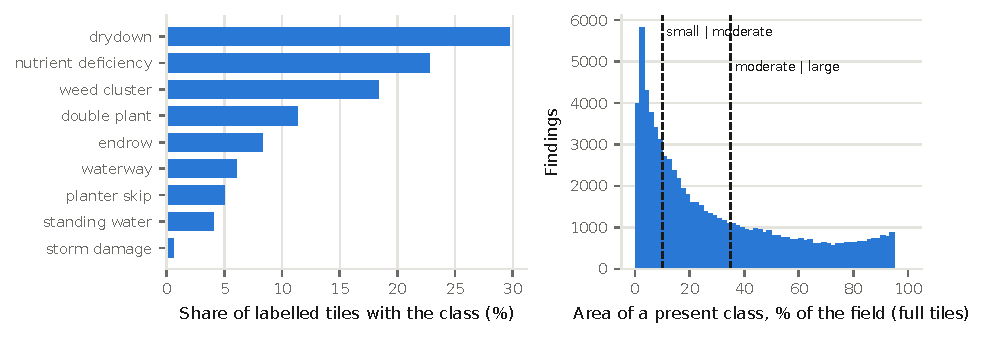
\includegraphics[width=\columnwidth]{figures/dataset.pdf}
\caption{The labelled data: share of tiles carrying each class (left), and the area of each present class with the extent cut points (right).}\label{fig:data}
\end{figure}

\paragraph{Mask statistics.} One streaming pass over the archive records, for each view and class, the class's share of in-field valid pixels and its share in each cell of a 3$\times$3 grid. Classes are counted independently, so overlapping labels count for both. A separate generator turns these statistics into pairs, so cut points can be retuned without re-reading the archive.

\paragraph{Question types.} All answers are short and closed-vocabulary:
\begin{itemize}
\item \emph{Presence} (``Is there weed cluster in this tile?''): yes / no. Each view asks about every class it contains and as many absent classes, chosen with a per-row seed, so yes and no are balanced.
\item \emph{Identify}: the classes present, largest first, or \emph{none}; scored as a set.
\item \emph{Extent}: small / moderate / large, with global cut points at 10\% and 35\% of in-field area (the rounded tertiles, 10.9\% and 37.4\%, of 72,661 full views).
\item \emph{Location}: the grid cell holding the most mask pixels, or \emph{throughout} when no cell holds 40\% of the mask.
\end{itemize}
Counting is excluded because the masks do not separate instances. Each type has fifteen hand-written templates: twelve for training and three, with name synonyms (``weeds'', ``standing water'') that no training template uses, held out for the paraphrase test. The first cycle trained on five (Section~\ref{sec:cycles}).

\paragraph{Captions.} Every present anomaly, largest first, with its extent and location, in one of 4--5 phrasings (``Large drydown throughout the tile, with a small weed cluster at the top left''). Targets end on their last word, with no full stop, for a reason the first cycle taught us (Section~\ref{sec:cycles}). Training samples one phrasing; BLEU and ROUGE score against all of them. Clean views read ``No anomalies visible''.

\paragraph{Ambiguous cases and hedges.} Ground truth is itself uncertain near the cut points, so we flag a pair as ambiguous when the area is within 12\% (relative) of an extent cut, when a present class covers under 1\% of the field, or when the top grid cell beats the runner-up by under 5 points or sits within 2.5 points of the 40\% \emph{throughout} cut. Flagged pairs train on a hedge: \emph{possibly}, \emph{small to moderate}, \emph{X or Y}.

\paragraph{Sampling.} Each training run draws pairs from a balanced sampler: a fixed mix of question types, class weights $\propto 1/\sqrt{\text{frequency}}$, presence yes/no 50/50 per class, and about 12\% clean quadrant views. Location draws keep the data's own mix of \emph{throughout} and grid-cell answers; Section~\ref{sec:cycles} reports what rebalancing them does. Loss is on answer tokens only.

\section{Method}\label{sec:method}
\paragraph{BLIP-LoRA.} Two checkpoints are adapted separately: \texttt{blip-vqa-base} for questions and \texttt{blip-image-captioning-base} for captions, both at 384 px. The base weights stay frozen in fp16 and the LoRA matrices train in fp32, with dropout 0.05, $\alpha = 2r$, AdamW, effective batch 16, a cosine schedule with 3\% warmup, gradient clipping at 1.0 and a loss scaler started at $2^{12}$.

\paragraph{Choosing rank, targets and learning rate.} On fold 0's inner validation set we change one setting at a time, keeping the best value before the next step: rank $\{4, 8, 16, 32, 64\}$ at LR $10^{-4}$ on attention query/value; then LR $\{5\!\times\!10^{-5}, 10^{-4}, 2\!\times\!10^{-4}, 5\!\times\!10^{-4}\}$; then targets \{text attention only, query/value in every attention layer, every linear layer\}. Each trial trains 10k pairs. The score is the mean accuracy over question types (fact F1 for captions), so the most numerous type cannot decide alone. Figure~\ref{fig:sweep} shows the second cycle's sweep: score rises with rank beyond 16, and both models prefer query/value adapters in every attention layer at rank 64 and LR $5\!\times\!10^{-4}$.

\paragraph{A learning rate that only works for short runs.} The sweep's 10k-pair trials decay the learning rate to zero within the run. Held near $5\!\times\!10^{-4}$ for up to 120k pairs, the VQA model failed in three of five folds (Figure~\ref{fig:lr}): two fell to 0.125, the score of giving one answer to everything, and fold 0 lost every identify answer at 20k pairs and ended at 0.56, against 0.66 at the capped rate. The sweep had scored $2\!\times\!10^{-4}$ within one point of $5\!\times\!10^{-4}$, so final runs cap the learning rate at $2\!\times\!10^{-4}$; no fold collapsed at the cap. We keep this as a finding: a short sweep can select a learning rate that a long run cannot survive.

\paragraph{Final runs and checkpoint choice.} Each fold trains the full 120k pairs and scores its inner validation set every 5k pairs. Validation swings while the learning rate is near its peak, so the kept checkpoint is the best of the second-half checks. Without this rule one caption fold kept a 5k-pair adapter with the best class F1 but correct locations for 1\% of its findings. The first cycle also stopped a fold after three checks without a new best; Section~\ref{sec:cycles} shows that rule fired on noise. From the third cycle on, runs are longer and validate on more tiles (Section~\ref{sec:length}).

\paragraph{Served model.} The laptop app needs a VLM that runs on a CPU. A bake-off trained three candidates on the same 10k pairs with identical LoRA settings (rank 16, $\alpha$ 32, every linear layer of the language model, LR $10^{-4}$): LFM2.5-VL-450M scored 0.469, LFM2.5-VL-1.6B 0.535 and Qwen3.5-2B 0.560, so Qwen3.5-2B won. Adding LoRA to its vision tower gained only 1.6 points, under our 2-point bar, so adapters stay on the language model and can be swapped per request at serving time. Two variants then train for 30k pairs each in the first cycle and, restarted from that checkpoint, 30k more on the second cycle's targets: one reads the RGB tile, the other also reads an NDVI map of the same view as a second image, coloured with a fixed ramp. The masks were drawn by annotators who looked at RGB, NIR and NDVI views, and NIR inputs improved the dataset paper's segmentation models~\cite{chiu2020agriculture}, which motivates the second variant.

\section{Evaluation protocol}\label{sec:eval}
\paragraph{Dynamic cross-validation.} Tiles from one field are highly correlated, so folds group by field: 5-fold \texttt{StratifiedGroupKFold} over the 75,278 tiles, grouped by field and stratified on each tile's rarest class, regenerated from a seed recorded at the start of every run and shared by every model in it. No split file is saved or reused. Each training fold holds out about 10\% of its fields as the inner validation set; test folds are never seen before final scoring.

\paragraph{Test sample.} Per fold, about 2,000 test tiles with at least 50 tiles of every class where available, their applicable pairs, every ambiguous pair, and 300 clean quadrant views: about 11,000 questions and 2,200 captions per fold. BLIP rows use all five folds (mean $\pm$ std); the served model uses fold 0, with 95\% intervals from a bootstrap that resamples whole test fields and paired differences on the same items.

\paragraph{Scoring.} The generated answer is normalised (case, punctuation, articles, plurals) and matched exactly; Identify is matched as a set. BLIP's headline readout ranks the question type's fixed answers by likelihood and returns the most likely one; it was chosen on validation (Section~\ref{sec:length}), and greedy generation is reported beside it. For the final model's headline, a correction for label shift, also chosen on validation, re-weighs the top two ranked answers (Section~\ref{sec:length}). Captions get BLEU-1/4, ROUGE-L and CIDEr against all phrasings, and \emph{fact} precision, recall and F1: class mentions parsed back out of the caption and compared with the masks. On ambiguous pairs a hedge scores 1, committing to either side 0.5, anything else 0; on clear pairs a hedge is wrong. Confidence is the geometric mean of the answer tokens' probabilities.

\section{Results}\label{sec:results}
\subsection{Zero-shot vs LoRA}
\begin{table*}[t]\centering\small
\resizebox{\textwidth}{!}{\begin{tabular}{lccccccccc}
\toprule
Model & Presence & Identify & Extent & Location & Mean & BLEU-4 & ROUGE-L & CIDEr & Fact F1 \\
\midrule
Zero-shot BLIP & 59.4 $\pm$ 1.4 (59.5) & 13.4 $\pm$ 0.1 (6.1) & 41.1 $\pm$ 1.2 (0.0) & 4.3 $\pm$ 0.7 (0.0) & 29.6 $\pm$ 0.4 (16.4) & 0.0 $\pm$ 0.0 & 9.8 $\pm$ 0.4 & 0.01 & 0.0 $\pm$ 0.0 \\
Most common answer & 53.3 $\pm$ 0.0 & 23.2 $\pm$ 4.0 & 35.7 $\pm$ 1.9 & 57.3 $\pm$ 2.0 & 42.4 $\pm$ 1.2 & -- & -- & -- & -- \\
BLIP-LoRA v1 & 89.9 $\pm$ 0.4 (89.9) & 59.3 $\pm$ 1.8 (56.5) & 60.6 $\pm$ 2.3 (61.0) & 60.9 $\pm$ 2.3 (59.6) & 67.7 $\pm$ 0.9 (66.8) & 14.9 $\pm$ 0.9 & 40.7 $\pm$ 1.7 & 0.13 & 58.3 $\pm$ 4.0 \\
BLIP-LoRA v2 & 90.5 $\pm$ 0.9 (90.5) & 60.4 $\pm$ 1.0 (56.8) & 60.3 $\pm$ 3.4 (59.7) & 61.0 $\pm$ 2.1 (60.1) & 68.1 $\pm$ 1.2 (66.8) & 56.2 $\pm$ 4.9 & 73.5 $\pm$ 2.6 & 3.49 & 76.8 $\pm$ 2.7 \\
BLIP-LoRA & 91.3 $\pm$ 1.0 (91.3) & 73.8 $\pm$ 2.7 (59.3) & 64.8 $\pm$ 2.4 (63.6) & 66.3 $\pm$ 1.5 (64.7) & 74.0 $\pm$ 1.3 (69.7) & 60.2 $\pm$ 0.7 & 76.3 $\pm$ 0.3 & 3.86 & 80.4 $\pm$ 0.9 \\
\bottomrule
\end{tabular}
}
\caption{The graded ablation: accuracy (\%) per question type on held-out folds, mean $\pm$ std over 5 field-grouped folds under the ranked readout, greedy generation in brackets, and caption metrics. v1 and v2 are the first and second cycles. \emph{Most common answer} gives the single best answer per question type, picked with hindsight on each fold's test items: the floor any model has to clear.}\label{tab:ablation}
\end{table*}

Table~\ref{tab:ablation} is the headline. Zero-shot BLIP answers presence a little above chance and, generating freely, almost never produces an extent or location in our vocabulary; even with its answers ranked over each type's list it stays below a constant answer (\zeroMean\% against \constMean\%). After fine-tuning, BLIP-LoRA reaches \blipMean\% mean accuracy under the ranked readout (\blipGreedy\% greedy; \blipCorrMean\% after the label-shift correction of Section~\ref{sec:length}), with a standard deviation of \blipMeanStd\ points across the five folds. The gains are uneven. Presence is nearly solved (\blipPresence\%); identify (\blipIdentify\%), extent (\blipExtent\%) and location (\blipLocation\%) are learned but far from it. Location gains least over its floor: most anomalies are spread out, so \emph{throughout} is right \constLocation\% of the time. Captions go from no correct facts to a fact F1 of \blipFactF\% (precision \blipFoldPrecision\%, recall \blipFoldRecall\% on fold 0). The table keeps the first two cycles' rows above the final one; Sections~\ref{sec:cycles} and~\ref{sec:length} explain the differences. CIDEr stays near zero because every caption shares one small template vocabulary, which CIDEr's document-frequency weighting discounts; fact F1 is the caption metric we rely on.

\begin{figure*}[t]\centering
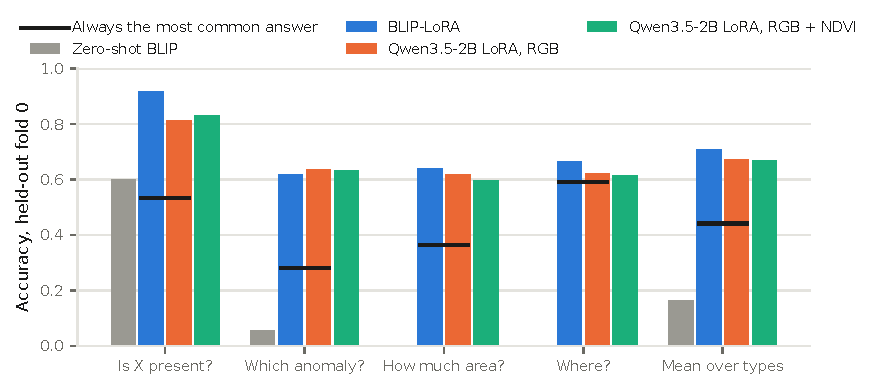
\includegraphics[width=\textwidth]{figures/family_bars.pdf}
\caption{Fold 0, the same 13,004 held-out items for every model. Bars: accuracy per question type; black ticks: the best constant answer.}\label{fig:bars}
\end{figure*}

\subsection{Choosing rank, target modules and learning rate}
\begin{figure*}[t]\centering
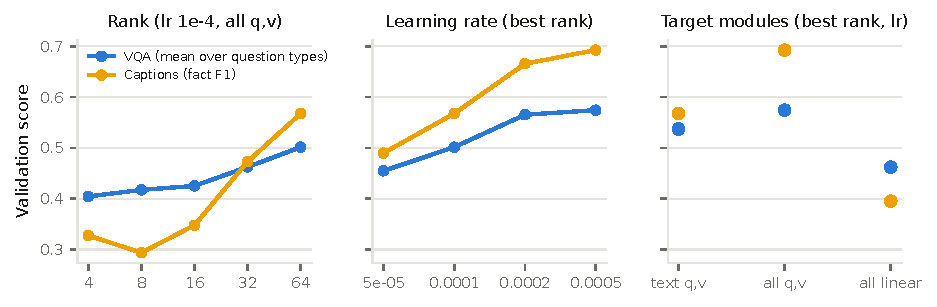
\includegraphics[width=\textwidth]{figures/sweep.pdf}
\caption{The LoRA sweep on fold 0's inner validation set, 10k pairs per trial, one setting at a time.}\label{fig:sweep}
\end{figure*}
\begin{figure*}[t]\centering
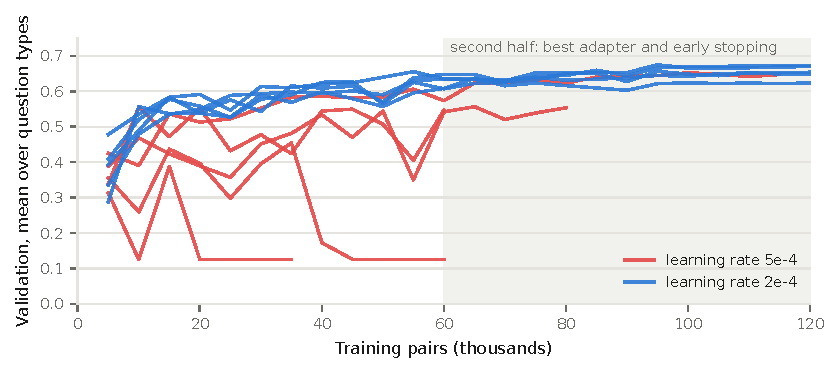
\includegraphics[width=\textwidth]{figures/lr_curves.pdf}
\caption{BLIP VQA validation over training, five folds each. At the sweep's $5\!\times\!10^{-4}$ (red) two folds collapse to a constant answer; at $2\!\times\!10^{-4}$ (blue) every fold trains smoothly. Shaded: the checks eligible for checkpoint choice and early stopping.}\label{fig:lr}
\end{figure*}
Rank is the clearest lever in a 10k-pair sweep (Figure~\ref{fig:sweep}): VQA validation rises from 0.404 at rank 4 to 0.502 at rank 64, captions from 0.328 to 0.568. Learning rate is the second: from $5\!\times\!10^{-5}$ to $5\!\times\!10^{-4}$ the models gain 0.12 and 0.20. Leaving the image encoder frozen (text attention only) costs 4 points on questions and 12 on captions, so the encoder has to adapt to aerial imagery, captions most of all. Adapting every linear layer hurts both at that learning rate (0.462 and 0.395 against 0.574 and 0.693 for query/value adapters). The first cycle's captions, whose targets the base model could not end, had preferred every linear layer; once targets ended cleanly, query/value adapters won for both tasks. The adapters train 11.8M parameters for VQA and 7.1M for captions.

\paragraph{LoRA or DoRA?} DoRA~\cite{liu2024dora} splits each adapted weight into a magnitude and a direction. Trained on fold 0 in the first cycle with that cycle's settings, it adds 0.1M parameters and 29\% training time (7.2 against 5.6 minutes per 5k pairs on a T4) and scores 72.2\% pooled accuracy against the first cycle's LoRA at 72.6\%, a paired difference of $-0.4$ points (95\% CI $-1.1$ to 0.3; Table~\ref{tab:fold0}, where it is paired with the ``v1'' LoRA row). Plain LoRA stays, and the second cycle did not retrain DoRA.

\subsection{Second cycle: four findings from the first}\label{sec:cycles}
The first full cycle of this project trained and scored everything in this report before we read its outputs closely. Reading them found four training-side faults, each with a measured cause. The second cycle addressed them and retrained the ten BLIP folds and the served variants on the same questions, cut points and ground truth, so every first-cycle score stays comparable, and the kept checkpoint is still scored with the first training phrasing of each type. Tables~\ref{tab:ablation} and~\ref{tab:fold0} keep the first cycle's rows, marked ``v1'', and the second cycle's, marked ``v2'', above the final ones. The zero-shot, DoRA and leakage records were not retrained and are first-cycle results.

\paragraph{Captions that never end.} First-cycle captions ran to \voneFoldWords\ words on average against \referenceWords\ in their references, with fact precision \voneFoldPrecision\% and recall \voneFoldRecall\%. The cause is in the base model: \texttt{blip-image-captioning-base} assigns a full stop a loss near 13 nats, so a target that ends in ``.'' asks for a token the adapters never make likely, and generation runs to the length limit, repeating findings. Caption targets now end on their last word (Table~\ref{tab:captions}). Fold 0's validation fact F1 rose from 0.631 to 0.839, and on the held-out items fact F1 goes from \voneFoldFactF\% to \blipFoldFactF\% (precision \voneFoldPrecision\% to \blipFoldPrecision\%, \voneFoldWords\ to \blipFoldWords\ words).
\begin{table*}[t]\centering\footnotesize
\begin{tabular}{lp{0.26\textwidth}p{0.26\textwidth}p{0.26\textwidth}}
\toprule
Tile & Reference & First cycle & Final \\
\midrule
Clean & No anomalies visible & visible here the tile the field looks clean the tile the field looks clean the tile the field has small nutrient deficiency at the bottom right or throughout the tile & the field looks clean \\
One finding & Small waterway at the left & moderate waterway throughout the tile, with small weed cluster at the top right or throughout the tile and small waterway at the right or throughout the tile & this tile shows moderate waterway throughout the tile \\
Several findings & Small double plant at the bottom right, with possibly small weed cluster at the bottom right & visible here the field has small double plant at the bottom right or bottom right, with small weed cluster at the bottom right or bottom right, with small planter skip at the bottom right or bottom right & this tile shows small double plant at the bottom right \\
\bottomrule
\end{tabular}

\caption{Three fold-0 tiles, the lowest row id of each kind: the reference caption beside the first cycle's caption and the final one.}\label{tab:captions}
\end{table*}

\paragraph{Early stopping on noise.} The first cycle stopped a fold when three consecutive second-half checks failed to beat the best. Every VQA fold stopped between 80k and 115k pairs, yet the last six checks of each sat within 0.6 to 3.4 points of one another, the sampling noise of a 300-tile validation set, and four folds stopped with their last check within one point of their best. The rule was reading noise as a plateau. The caption folds, whose unterminated outputs made validation swing by up to eleven points, stopped between 75k and 85k. Final folds train their full 120k pairs and keep the best second-half check.

\paragraph{Location: do not rebalance the draws.} 55\% of location truths are \emph{throughout}, and the first cycle's model answered \emph{throughout} for 68\% of the items whose truth is a grid cell: on fold 0 it scored \voneLocThroughout\% on the \locNThroughout\ \emph{throughout} items and \voneLocLocalised\% on the \locNLocalised\ localised ones. The obvious fix is to draw more location questions whose answer is a cell, so one fold-0 run drew cells 65\% of the time (``balanced location draws'' in Table~\ref{tab:fold0}). It moved accuracy from the majority to the minority: localised items went from \voneLocLocalised\% to \balLocLocalised\% and \emph{throughout} items from \voneLocThroughout\% to \balLocThroughout\%, and on the natural mix, where 55\% of questions keep the majority answer, its location accuracy ended \balLocDrop\ points below the second cycle's \vtwoFoldLocation\%. The second cycle and the final model keep the data's own draws (\vtwoLocThroughout\% and \blipLocThroughout\% on \emph{throughout} items, \vtwoLocLocalised\% and \blipLocLocalised\% on localised ones): a sampler that reweights the answer prior trades accuracy on the questions people ask for accuracy on the ones they do not, and the app's users ask about real tiles. Both adapters are kept, so a reader who needs localisation can take the other one.

\paragraph{Twelve phrasings.} The first cycle lost \voneParaphraseDrop\ points on held-out question wordings with five training templates per type. The second trains on twelve, none sharing a synonym with the three held-out ones, and loses \vtwoParaphraseDrop\ on the same items, barely less. Training longer did more: the final model loses \blipParaphraseDrop\ (Section~\ref{sec:robust}).

\subsection{What raised the ceiling: a study, then four doublings of length}\label{sec:length}
\begin{table}[t]\centering\scriptsize
\resizebox{\columnwidth}{!}{\begin{tabular}{rlccc}
\toprule
Pairs & Change from the reference & Validation & $\Delta$ [95\% CI] & Trainable (M) \\
\midrule
30k & the reference recipe & 58.2 & -- & 11.8 \\
30k & lr 0.0001, targets all\_linear & 59.0 & +0.8 [+0.0, +1.6] & 40.1 \\
30k & targets all\_linear & 59.9 & +1.7 [+0.7, +2.8] & 40.1 \\
30k & alpha 64 & 57.2 & $-$1.0 [$-$1.9, $-$0.2] & 11.8 \\
30k & alpha 256 & 59.0 & +0.8 [$-$0.1, +1.5] & 11.8 \\
30k & dropout 0.0 & 58.3 & +0.1 [$-$0.5, +0.6] & 11.8 \\
30k & dropout 0.1 & 58.0 & $-$0.2 [$-$0.6, +0.2] & 11.8 \\
30k & dropout 0.2 & 58.2 & +0.0 [$-$0.5, +0.4] & 11.8 \\
30k & train\_norms True & 57.8 & $-$0.4 [$-$1.1, +0.2] & 12.0 \\
30k & bands nrg & 57.1 & $-$1.1 [$-$2.3, +0.2] & 11.8 \\
30k & rank 128, alpha 256 & 58.9 & +0.7 [+0.0, +1.4] & 23.6 \\
30k & rank 256, alpha 512 & 59.5 & +1.3 [+0.5, +2.1] & 47.2 \\
30k & rank 256, alpha 512, seed 1 & 59.5 & +1.3 [+0.0, +2.7] & 47.2 \\
30k & seed 1 & 57.6 & $-$0.6 [$-$2.0, +0.8] & 11.8 \\
30k & seed 2 & 56.5 & $-$1.7 [$-$3.1, $-$0.4] & 11.8 \\
30k & size 512 & 58.2 & $-$0.0 [$-$0.9, +0.8] & 11.8 \\
60k & the reference recipe & 60.8 & +2.6 [+1.5, +3.8] & 11.8 \\
120k & targets all\_linear (vs 120k) & 63.4 & +0.8 [$-$0.3, +1.8] & 40.1 \\
120k & the reference recipe & 62.6 & +4.4 [+2.7, +6.3] & 11.8 \\
120k & seed 1 (vs 120k) & 61.2 & $-$1.4 [$-$3.0, +0.1] & 11.8 \\
120k & rank 256, alpha 512 (vs 120k) & 63.2 & +0.6 [$-$0.7, +1.9] & 47.2 \\
240k & the reference recipe & 63.7 & +5.5 [+3.6, +7.8] & 11.8 \\
480k & the reference recipe & 65.1 & +6.9 [+5.2, +8.8] & 11.8 \\
\bottomrule
\end{tabular}

}
\caption{The VQA study on fold 0's 1,000 inner-validation tiles: mean over question types (\%), greedy readout, and the paired change against the reference recipe at the same length (``vs 120k'': against the 120k reference) with a field-grouped 95\% interval. The interval covers item sampling, not training noise: three seeds of the reference span 56.5 to 58.2.}\label{tab:study}
\end{table}
\paragraph{The study.} After the second cycle we changed one setting at a time from its VQA recipe (rank 64, $\alpha$ 128, LR $2\!\times\!10^{-4}$, query/value adapters, dropout 0.05, 384 px), trained 30k pairs per trial on fold 0, and scored 1,000 inner-validation tiles (Table~\ref{tab:study}). Three training seeds of the unchanged recipe spread from 56.5 to 58.2, so one 30k run carries about a point of noise that the field bootstrap does not see. Capacity gained a little at 30k: rank 256 by 1.3 points under two seeds, adapters on every linear layer by 1.7 at 3.4 times the trainable parameters. Neither gain held at 120k pairs, where rank 256 adds 0.6 (95\% CI $-0.7$ to 1.9) and every linear layer 0.8 ($-0.3$ to 1.8), less than the 1.4 points between two seeds of the same recipe. Dropout, $\alpha$, training the LayerNorms, 512-pixel inputs and a near-infrared--red--green image stayed within seed noise. BLIP-large captioning matched the base model (fact F1 71.9 against 72.1) at four times the compute, and no BLIP-large VQA checkpoint exists, so the base model stays. Length was the one lever far outside the noise: +2.6 points at 60k pairs, +4.4 at 120k, +5.5 at 240k and +6.9 at 480k.

\paragraph{Reading out the answer.} Instead of generating an answer, the model can score every answer in the question type's fixed list and return the most likely. On the second cycle's fold-0 adapters and validation tiles, ranking gains 1.1 points over greedy generation (95\% CI 0.4 to 1.8), mostly on identify, while beam search of width 3 loses 0.2. Ranking can only return a well-formed answer, so it is the headline readout from here on. Two other ways to spend compute at test time did less than training longer: averaging predictions over flipped and rotated views changed nothing ($+0.0$, $-0.5$ to 0.5), and averaging two 120k seeds gained 0.8 points over one seed, against 1.9 for spending the same doubling on length.

\begin{table*}[t]\centering\small
\resizebox{\textwidth}{!}{\begin{tabular}{crcccccc}
\toprule
Cycle & Pairs & Validation & Held out, ranked & Change [95\% CI], folds up & Held out, greedy & Partial credit & Perturbed images \\
\midrule
2 & 120k & -- & 68.1 $\pm$ 1.2 & -- & 66.8 $\pm$ 1.1 & 72.7 $\pm$ 1.2 & $-3.9$ \\
3 & 240k & 68.2 & 70.2 $\pm$ 1.2 & +2.2 [+1.1, +3.2], 5/5 & 68.8 $\pm$ 1.4 & 74.7 $\pm$ 1.0 & $-4.9$ \\
4 & 480k & 69.5 & 71.5 $\pm$ 1.6 & +1.3 [+0.7, +1.9], 5/5 & 69.6 $\pm$ 1.5 & 76.0 $\pm$ 1.5 & $-5.0$ \\
5 & 960k & 71.5 & 73.1 $\pm$ 1.6 & +1.6 [+0.8, +2.3], 5/5 & 70.2 $\pm$ 1.1 & 77.5 $\pm$ 1.5 & $-6.9$ \\
\bottomrule
\end{tabular}
}
\caption{Training length, five field-grouped folds per cycle (\%). Validation is the selection score: each fold's best second-half check, averaged over folds (cycle 2 validated on a different draw). Held out: mean $\pm$ sd over folds of the four-question mean. Change: against the cycle before, with a paired $t$ interval over folds and the number of folds that improved. Captions use cycle 2's adapters in these rows. Perturbed images: the change in greedy accuracy on fold 0's 500 robustness tiles, averaged over the seventeen image perturbations of Figure~\ref{fig:robust}.}\label{tab:cycles}
\end{table*}
\begin{figure}[t]\centering
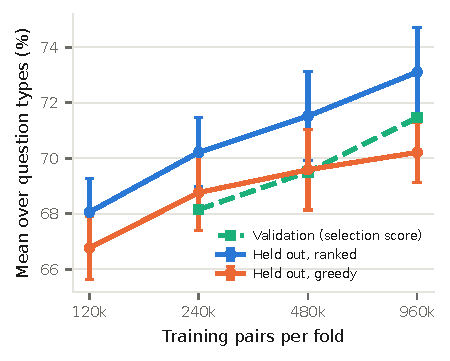
\includegraphics[width=\columnwidth]{figures/length_curve.pdf}
\caption{Held-out four-question mean (mean and sd over five folds) under both readouts, and the validation score that chose each cycle, against training pairs per fold.}\label{fig:length}
\end{figure}
\paragraph{Cycles 3 to \finalCycle.} Each cycle doubles the training pairs of the second cycle's VQA recipe. Each new length trains fold 0 first, and the other folds follow only if fold 0's validation rises. Each fold scores 1,000 inner-validation tiles, drawn by the held-out sample's rules, six times during training and keeps the best second-half check under the ranked readout. A rule fixed before any of these cycles' held-out scores were read picks the final cycle: the highest mean validation over its five folds. Held-out scores never choose. Table~\ref{tab:cycles} and Figure~\ref{fig:length} show validation and held-out scores rising together. The rule chose cycle \finalCycle\ (\finalPairs\ pairs; validation \finalVal\ against \prevVal\ for the cycle before). It scores \blipMean\% held out, \finalChange\ points more than the cycle before (95\% CI \finalChangeLo\ to \finalChangeHi, \finalChangeFolds\ of 5 folds up) and \totalChange\ more than cycle 2 (\totalChangeLo\ to \totalChangeHi). Greedy generation gains less from length (\blipGreedy\% for the final model). One untested reading is that longer training sharpens the answer likelihoods that ranking reads more than it changes the string greedy decoding emits. Length was not free: the table's last column shows each cycle more fragile to damaged images (Section~\ref{sec:robust}).

\paragraph{Captions at 480k pairs.} Cycle 2's caption runs were still at their best when they ended, so fold 0 trained captions for 480k pairs: validation fact F1 rose from 78.3 to 81.1, with BLEU-4 and ROUGE-L also up. The other folds followed, and the final model pairs these caption adapters with the chosen cycle's VQA adapters. Held out, fact F1 goes from \vtwoFactF\% to \blipFactF\% (fold-paired change \capChange\ points, 95\% CI \capChangeLo\ to \capChangeHi, \capChangeFolds\ of 5 folds up), and the VQA answers are unchanged.

\paragraph{Correcting for label shift.} Training draws are balanced (Section~\ref{sec:data}), while validation and test follow the held-out sample's rules, where common classes fill the sample. The ranked readout carries the training mix with it: over the five validation sets, nutrient deficiency is the true identify answer \corrNdTrue\ times but the ranked answer only \corrNdSaid\ times, and it is often the runner-up. We adjust for this label shift as \cite{saerens2002adjusting} do, estimating the shift from the readout's own confusion on validation, in the spirit of \cite{lipton2018detecting}. For each question type and answer, a ratio of (times answered $+1$) to (times true $+1$) is taken on the fold's own validation set. The two ranked answers each record stores have their probabilities divided by ratio$^w$, and the larger wins; $w$ is chosen per question type on the same set from $\{0, 0.5, 1, 2, 3, 5\}$. Fitted on one field-grouped half of each fold's validation and scored on the other half, the correction gains \corrValChange\ points (95\% CI \corrValLo\ to \corrValHi, \corrValFolds\ of 5 folds up), all of it on identify. A rule fixed before the held-out read therefore made it the final readout. Held out, it lifts the four-question mean from \blipMean\% to \textbf{\blipCorrMean\%} (\corrChange\ points, \corrChangeLo\ to \corrChangeHi, \corrChangeFolds\ of 5 folds up) and identify from \blipIdentify\% to \corrIdentify\%. The other question types keep $w$ at or near 0 and do not move. The other readout change we tried, hedging between the top two answers when their probabilities are close, lost on validation at every margin.

\subsection{Hedging on ambiguous cases}
\begin{table*}[t]\centering\small
\resizebox{\textwidth}{!}{\begin{tabular}{lccccccc}
\toprule
Model & Hedge, amb. & Hedge, clear & Credit, amb. & Acc., clear & ECE & AURC & Acc. at 80\% cov. \\
\midrule
Zero-shot BLIP & 0.0 & 0.0 & 1.0 & 27.1 & 0.232 & 0.535 & 31.2 \\
BLIP-LoRA & 2.2 & 0.5 & 39.9 & 77.3 & 0.134 & 0.082 & 83.9 \\
Qwen3.5-2B LoRA, RGB & 0.0 & 0.0 & 37.3 & 72.1 & 0.118 & 0.145 & 75.1 \\
Qwen3.5-2B LoRA, RGB + NDVI & 0.0 & 0.0 & 36.7 & 72.2 & 0.109 & 0.145 & 75.2 \\
BLIP-DoRA v1 & 0.0 & 0.0 & 36.8 & 74.1 & 0.141 & 0.098 & 80.7 \\
\bottomrule
\end{tabular}
}
\caption{Hedging and calibration on fold 0 under greedy generation, whose words could hedge (\%, except ECE and AURC). Hedge rates are the share of answers that hedge; credit on ambiguous pairs gives 0.5 for committing to one side. AURC: area under the risk--coverage curve, lower is better.}\label{tab:hedging}
\end{table*}
No model hedges in words (Table~\ref{tab:hedging}). Hedged targets are only about a tenth of extent and location pairs and rarer elsewhere, so a committed answer is always the more likely one; on ambiguous pairs fine-tuned BLIP earns \blipCreditAmb\% partial credit against \blipAccClear\% accuracy on clear ones. The hedging signal lives in the confidence instead (Figure~\ref{fig:rc}). Answering only the most confident 80\% of questions raises BLIP-LoRA's share of fully correct answers from \blipAccAll\% to \blipAccEighty\%, and its AURC falls from \zeroAurc\ zero-shot to \blipAurc. The served app therefore reports a confidence with every finding rather than relying on hedged wording.

\begin{figure}[t]\centering
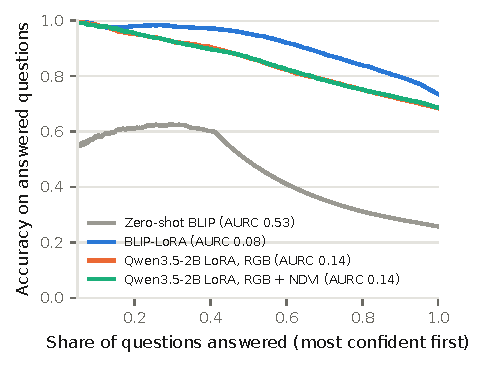
\includegraphics[width=\columnwidth]{figures/risk_coverage.pdf}
\caption{Selective answering on fold 0: accuracy on the most confident share of questions.}\label{fig:rc}
\end{figure}

\subsection{Robustness}\label{sec:robust}
\begin{figure*}[t]\centering
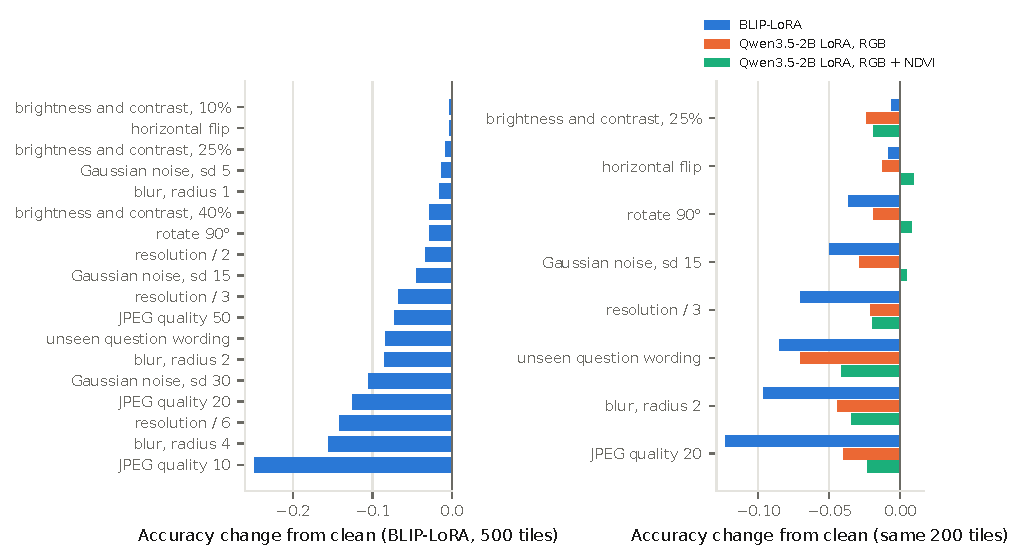
\includegraphics[width=\textwidth]{figures/robustness.pdf}
\caption{Accuracy change from clean on fold 0. Left: BLIP-LoRA on the 500-tile robustness subset, every perturbation and strength. Right: all three fine-tuned models on its first 200 tiles, at the middle strength of each perturbation.}\label{fig:robust}
\end{figure*}
Fine-tuned BLIP barely moves under lighting changes (\blipLightDrop\ points at the strongest) or a flip (\blipFlipDrop), and loses \blipRotDrop\ to a quarter-turn once location answers are remapped (Figure~\ref{fig:robust}). It degrades smoothly with blur, noise and lost resolution, and sharply with heavy JPEG compression ($-$\blipJpegDrop\ at quality 10). Question wording is the one drop that shrank. On held-out templates and synonyms the first cycle's model lost \voneParaphraseDrop\ points, the second \vtwoParaphraseDrop\ and the final model \blipParaphraseDrop\ (Section~\ref{sec:cycles}). Zero-shot BLIP barely moves under any perturbation, but only because it is near its floor everywhere.

\paragraph{Length costs robustness.} Each doubling of training that raised held-out accuracy also made the model more fragile to damaged images. Averaged over the seventeen image perturbations, the accuracy change on fold 0 goes from $-$\vtwoPerturbed\ points at 120k pairs to $-$\blipPerturbed\ at \finalPairs\ (Table~\ref{tab:cycles}, last column). At JPEG quality 10 the second cycle's model loses \vtwoJpegDrop\ points and the final one \blipJpegDrop. The final model starts higher on clean tiles (\blipRobustClean\% against \vtwoRobustClean\%, greedy) and ends lower (\blipJpegAcc\% against \vtwoJpegAcc\%). The first cycle's model, trained as long as the second on the old data scheme, loses \vonePerturbed\ on average, so the fragility follows length rather than the second cycle's fixes. Training applies no image augmentation; one reading is that the extra passes fit the texture and compression of clean tiles. Training on perturbed copies would test it, and we have not run it.

On the first 200 robustness tiles, which Qwen3.5-2B was also scored on (Figure~\ref{fig:robust}, right), Qwen loses \servedRgbParaphraseDrop\ points to new wording (RGB) and \servedNdviParaphraseDrop\ (NDVI): its language model has met far more ways of asking a question than our templates. Damaged images cost Qwen less than BLIP. At the middle strengths JPEG compression costs BLIP \blipMidJpeg\ points against \servedRgbMidJpeg\ (RGB) and \servedNdviMidJpeg\ (NDVI), blur \blipMidBlur\ against \servedRgbMidBlur\ and \servedNdviMidBlur, and lost resolution \blipMidRes\ against \servedRgbMidRes\ and \servedNdviMidRes. Brightness is the exception: it leaves BLIP almost untouched (\blipMidLight) and costs each Qwen variant about two points (\servedRgbMidLight\ and \servedNdviMidLight).

\subsection{Does the official split leak?}
The official train and validation splits share fields: 480 of 2,116 fields have flights in more than one split. If a model memorised fields, its scores on official validation tiles from those fields would be inflated. We train one BLIP-LoRA VQA model on the official train split with the first cycle's settings (its early stopping fired at 115k pairs) and score official validation tiles from the 201 fields that also appear in training and from 250 that do not, sampled like the test sample (Table~\ref{tab:leak}).

\begin{table}[t]\centering\small\emph{Pending: the official-split run is still training.}

\caption{Leakage test: one model trained on the official train split, scored on official validation tiles. The interval on the difference resamples the fields of each half independently.}\label{tab:leak}\end{table}

Seen-field tiles score 2.3 points \emph{lower} than unseen-field tiles, with a 95\% interval of $-6.5$ to 2.2: no detectable inflation, and any inflation above about 2 points is ruled out. The shared fields recur on different flights, and the anomalies themselves can change between flights (drydown, weeds and standing water come and go), so having seen a field does not give away its labels. The overlap is real but harmless for this task. We still group folds by field: it costs nothing, and it keeps the comparison honest for tasks where a field's appearance does give away the answer.

\subsection{Where does the model look?}
For ``Is there \emph{X} in this tile?'' on 300 held-out tiles we take BLIP's last text-encoder cross-attention, weight it by the gradient of the answer's log-probability~\cite{selvaraju2017gradcam}, and score the resulting 24$\times$24 map against the class mask. Fine-tuning moves the attention peak inside the anomaly in \pointLora\% of cases, against \pointZero\% zero-shot and \pointChance\% expected by chance (the pointing game~\cite{zhang2018topdown}), and puts \energyLora\% of the positive attention energy on the mask, against \energyZero\% zero-shot. Fine-tuning taught BLIP to look at the anomaly more often, though far from always.

\subsection{The served model and the NDVI comparison}
\begin{table*}[t]\centering\small
\resizebox{\textwidth}{!}{\begin{tabular}{lcccccccc}
\toprule
Model & Presence & Identify & Extent & Location & Mean & Pooled acc. [95\% CI] & $\Delta$ vs BLIP-LoRA & Fact F1 (P/R) \\
\midrule
Zero-shot BLIP & 60.1 & 5.4 & 0.0 & 0.0 & 16.4 & 25.8 [24.6, 26.9] & -49.4 [-52.3, -46.6] & 0.0 (0/0) \\
BLIP-LoRA v1 & 90.5 & 58.2 & 60.3 & 61.9 & 67.7 & 72.6 [70.2, 75.0] & -2.6 [-3.9, -1.5] & 61.3 (46/92) \\
BLIP-LoRA v2 & 90.6 & 57.2 & 59.4 & 63.3 & 67.6 & 72.5 [70.2, 75.1] & -2.6 [-3.8, -1.6] & 77.3 (76/79) \\
BLIP-LoRA & 92.1 & 59.9 & 64.5 & 66.0 & 70.6 & 75.2 [72.8, 77.7] & -- & 80.3 (78/82) \\
BLIP-DoRA v1 & 90.5 & 55.9 & 59.7 & 62.9 & 67.2 & 72.2 [69.9, 74.6] & -0.4 [-1.1, 0.3] & 61.2 (46/92) \\
BLIP-LoRA v2, balanced location draws & 91.0 & 57.2 & 61.8 & 56.0 & 66.5 & 71.7 [69.6, 74.1] & -0.8 [-1.6, -0.1] & 77.3 (76/79) \\
Qwen3.5-2B, zero-shot & 0.0 & 0.0 & 0.0 & 0.0 & 0.0 (14.2) & 0.0 [0.0, 0.0] & -75.2 [-77.7, -72.8] & 0.1 (100/0) \\
Qwen3.5-2B LoRA, RGB v1 & 72.4 & 58.8 & 57.9 & 62.1 & 62.8 & 64.9 [62.7, 67.2] & -10.3 [-11.8, -8.8] & 56.4 (58/55) \\
Qwen3.5-2B LoRA, RGB & 81.4 & 63.6 & 61.9 & 62.1 & 67.3 & 70.3 [68.2, 72.7] & -4.9 [-6.3, -3.4] & 64.9 (66/64) \\
Qwen3.5-2B LoRA, RGB + NDVI v1 & 76.9 & 59.1 & 58.7 & 62.9 & 64.4 & 67.1 [65.1, 69.3] & -8.1 [-9.6, -6.6] & 60.6 (60/61) \\
Qwen3.5-2B LoRA, RGB + NDVI & 83.1 & 63.4 & 59.6 & 61.5 & 66.9 & 70.4 [68.2, 72.7] & -4.8 [-6.5, -3.2] & 65.5 (63/68) \\
\midrule
NDVI minus RGB & \multicolumn{6}{c}{} & 0.1 [-0.8, 0.9] & \\
\bottomrule
\end{tabular}
}
\caption{Every model on the same fold-0 items (\%): accuracy per question type, pooled accuracy with a field-grouped 95\% interval, the paired difference against BLIP-LoRA, and caption fact F1 with precision and recall; a mean in brackets is the lenient readout of free-text answers. Rows marked v1 are the first cycle's records on the same items; BLIP-DoRA, trained only in the first cycle, is paired with the v1 LoRA row. The last row is the paired NDVI minus RGB difference.}\label{tab:fold0}
\end{table*}
\begin{table}[t]\centering\small
\resizebox{\columnwidth}{!}{\begin{tabular}{lrccc}
\toprule
Class & Present & BLIP-LoRA & Qwen, RGB & Qwen, RGB + NDVI \\
\midrule
double plant & 219 & 88.8 & 79.6 & 78.7 \\
drydown & 624 & 97.3 & 84.6 & 91.6 \\
endrow & 139 & 80.7 & 80.0 & 78.4 \\
nutrient deficiency & 394 & 94.4 & 72.4 & 78.6 \\
planter skip & 89 & 89.7 & 77.4 & 79.1 \\
storm damage$^\dagger$ & 53 & 26.2 & 57.4 & 50.0 \\
standing water & 100 & 96.9 & 90.9 & 87.7 \\
waterway & 145 & 86.5 & 81.2 & 80.7 \\
weed cluster & 302 & 88.2 & 71.9 & 71.2 \\
\bottomrule
\end{tabular}
}
\caption{Presence F1 (\%) per class on fold 0. $^\dagger$Under 60 present examples.}\label{tab:perclass}
\end{table}
Table~\ref{tab:fold0} puts every model on the same 13,004 items. Zero-shot Qwen3.5-2B scores zero under exact match because it answers in full sentences (``No, there is no endrow visible in this tile\ldots''); a lenient readout that takes the leading yes or no, the class names, the extent word or the cell word from the sentence gives it 14.2\%, with presence at chance (49\%), so like BLIP it has no usable zero-shot knowledge of these anomalies. The lenient readout changes no fine-tuned model's score. After 60k pairs the RGB variant reaches \qwenRgbPooled\% pooled accuracy and the NDVI variant \qwenNdviPooled\%. Overall the NDVI map changes accuracy by \ndviDiff\ points (95\% CI \ndviLo\ to \ndviHi). Per class it helps where plant physiology says it should (Table~\ref{tab:perclass}): presence F1 rises for drydown (+7.0) and nutrient deficiency (+6.1), the anomalies that change how much a plant reflects in the near infrared, and moves by under 2 points for five of the other seven; water falls by 3.2 and storm damage, with 53 examples, by 7.4. After the first cycle's 30k pairs the NDVI variant had also led on waterway and endrow and trailed on weed clusters; the second cycle's 30k more pairs closed those gaps.

Qwen's paired difference against BLIP-LoRA on the same items, greedy on both sides since Qwen generates its answers, is \qwenNdviDiff\ points (NDVI) and \qwenRgbDiff\ (RGB), and its caption precision is \qwenNdviPrecision\% against BLIP's \blipFoldPrecision\%. Most of the gap is presence (\qwenRgbPresence\% against \blipFoldPresence\%); on the other three types Qwen is within a few points of BLIP's greedy answers. Qwen trained on 60k pairs shared between captions and all four question types, while each BLIP VQA model trains on \finalPairs\ questions.

\section{Cost and system}\label{sec:system}
\begin{table}[t]\centering\small
\resizebox{\columnwidth}{!}{\begin{tabular}{lrrlr}
\toprule
Runs & Count & Trainable params (M) & GPU & GPU-hours \\
\midrule
BLIP VQA LoRA, 5 folds & 5 & 11.8 & T4 & 10.7 \\
BLIP caption LoRA, 5 folds & 5 & 7.1 & T4 & 8.6 \\
BLIP sweeps, 20 trials & 20 & -- & T4 & 3.3 \\
Leakage model (official split) & 1 & 11.8 & T4 & 2.2 \\
BLIP VQA DoRA, fold 0 & 1 & 11.9 & T4 & 2.4 \\
Served bake-off, 4 runs & 4 & -- & T4 & 6.6 \\
Qwen3.5-2B LoRA, RGB & 2 & 16.8 & T4 & 14.5 \\
Qwen3.5-2B LoRA, RGB + NDVI & 2 & 16.8 & RTX PRO 5000 / T4 & 20.0 \\
BLIP study, fold 0 & 31 & -- & RTX PRO 5000 & 20.1 \\
BLIP VQA cycle 3, 240k pairs & 5 & 11.8 & RTX PRO 5000 & 11.7 \\
BLIP VQA cycle 4, 480k pairs & 5 & 11.8 & RTX PRO 5000 & 20.0 \\
BLIP VQA cycle 5, 960k pairs & 5 & 11.8 & RTX PRO 5000 & 39.6 \\
BLIP VQA cycle 6, 1,920k pairs & 1 & 11.8 & RTX PRO 5000 & 4.3 \\
BLIP caption LoRA, 480k pairs & 5 & 7.1 & RTX PRO 5000 & 14.5 \\
\bottomrule
\end{tabular}
}
\caption{What each group of training runs cost, from the run logs: trainable parameters (``--'' where the group mixes settings), the GPU, and GPU-hours including validation. Runs that shared the workstation GPU each count their own wall-clock hours. Scoring and robustness suites add about 15 T4 GPU-hours.}\label{tab:cost}
\end{table}
Table~\ref{tab:cost} is the compute budget. The first two cycles, the sweeps, the analyses and most of the served model took about \tfourHours\ T4 GPU-hours of free Colab and Kaggle time, resumed across session limits through a private Hugging Face repository of checkpoints. The study and the length cycles ran on a shared workstation GPU (RTX PRO 5000, 48 GB), several runs at a time, for \proHours\ GPU-hours.

The app runs on a laptop CPU. A FastAPI backend serves the Qwen3.5-2B Q4\_K\_M GGUF through llama.cpp, with both trained adapters (34 MB fp16 LoRA GGUFs each) loaded at start and selected per request, and zero-shot BLIP on CPU for comparison. Images are capped at 144 tokens, the training budget. On the laptop, reading a held-out tile takes about 4 s with the RGB adapter and 7 s with the NDVI adapter, which encodes two images; switching adapters between requests costs nothing, and the same request returns the same caption after a switch. The web interface is a full-screen map with a drag-to-select field box and one chat panel: the user asks about a tile, sees the RGB and NDVI views, and gets a caption, structured findings with confidences, and answers streamed as they are generated. A context panel adds free satellite context for the selected box (Sentinel-2 NDVI from Planetary Computer, the HLS season series from NASA titiler-cmr, weather from NASA POWER); this context is shown to the user and is never model input, because at 10--30 m per pixel it cannot resolve the anomalies.

\section{Limitations}
BLIP reads RGB only, while the annotators also saw near infrared. Extent is our only severity signal, and its cut points are global rather than per class. Captions come from templates, so overlap metrics reward template matching. The served-model rows use fold 0 only, and NDVI from these cameras is relative, not calibrated. Location stays the weakest type, and paraphrased questions still cost \blipParaphraseDrop\ points. The leakage test uses one model and one split, and the DoRA and leakage results come from the first cycle. The served model trained mostly on free T4 GPUs, which bounded it to 60k pairs over two cycles. The 480k-pair caption adapters were chosen on fold 0's validation alone, without a rule fixed in advance. The label-shift correction re-weighs only the two answers each record stores, and it estimates the shift from the readout's own confusion on validation rather than from known class priors; training on draws that match the test's mix may do better and was not tried.\pending{length ceiling sentence after cycle 6}

\section{Conclusion}
Masks can be turned into language that a small VLM learns to read: LoRA lifts BLIP from below a constant-answer floor to \blipCorrMean\% of questions right on unseen fields, with calibrated confidence that supports abstaining. After the fixes, the largest gain came from training longer, not from capacity: rank, target modules, input size and a larger model stayed inside seed noise once runs were long, while each doubling of length raised validation and held-out scores together. The last gain came from reading the answers rather than training for them: correcting the ranking for the gap between balanced training draws and the test's class mix added \corrChange\ points, all on identify. Reading the first cycle's outputs was worth as much as training them: a base model that cannot end a sentence, an early-stopping rule that read noise as a plateau, a sampler fix that moved accuracy to the questions nobody asks, and too few training phrasings, each found by measurement and addressed without touching the ground truth, though twelve phrasings barely narrowed the paraphrase gap and longer training narrowed it more. A learning rate that wins a short sweep can fail a long run, the fields shared by the official split turned out harmless, and a near-infrared view helps exactly the anomalies it should. A general-purpose language model also shrugs off rephrased questions and damaged images more easily than a template-trained BLIP. Length had a price: each doubling made BLIP more fragile to damaged images, and under heavy JPEG compression the final model is less accurate than the 120k one.

\begin{thebibliography}{9}\small
\bibitem{chiu2020agriculture} M.~T. Chiu et al. Agriculture-Vision: A large aerial image database for agricultural pattern analysis. CVPR, 2020.
\bibitem{li2022blip} J.~Li, D.~Li, C.~Xiong, S.~Hoi. BLIP: Bootstrapping language-image pre-training for unified vision-language understanding and generation. ICML, 2022.
\bibitem{hu2022lora} E.~J. Hu et al. LoRA: Low-rank adaptation of large language models. ICLR, 2022.
\bibitem{kuckreja2024geochat} K.~Kuckreja et al. GeoChat: Grounded large vision-language model for remote sensing. CVPR, 2024.
\bibitem{selvaraju2017gradcam} R.~R. Selvaraju et al. Grad-CAM: Visual explanations from deep networks via gradient-based localization. ICCV, 2017.
\bibitem{zhang2018topdown} J.~Zhang et al. Top-down neural attention by excitation backprop. IJCV, 2018.
\bibitem{liu2024dora} S.-Y. Liu et al. DoRA: Weight-decomposed low-rank adaptation. ICML, 2024.
\bibitem{saerens2002adjusting} M.~Saerens, P.~Latinne, C.~Decaestecker. Adjusting the outputs of a classifier to new a priori probabilities: a simple procedure. Neural Computation, 14(1), 2002.
\bibitem{lipton2018detecting} Z.~C. Lipton, Y.-X. Wang, A.~J. Smola. Detecting and correcting for label shift with black box predictors. ICML, 2018.
\end{thebibliography}

\end{document}
